\documentclass[a4paper,12pt]{article}
\usepackage[utf8]{ inputenc}
\usepackage[ngerman]{babel}
\usepackage[a4paper, left=2.5cm, right=2.5cm]{geometry}
\usepackage{graphicx}
\usepackage{subcaption}
\usepackage{fancyhdr}
\usepackage{pdfpages}
\usepackage{listings}
\usepackage{hyperref}
\usepackage[official]{eurosym}
\usepackage{float}

\pagestyle{fancy}
\lstset{
	language=Matlab,
	breaklines=true,
	morekeywords={matlab2tikz},
	keywordstyle=\color{blue},
	morekeywords=[2]{1}, keywordstyle=[2]{\color{black}},
	identifierstyle=\color{black},
	stringstyle=\color{mylilas},
	commentstyle=\color{mygreen},
	showstringspaces=false,
	mathescape=true
	emph=[1]{for,end,break},emphstyle=[1]\color{red},
}

\lhead{Investitionsrechnung für Haushalte}
\chead{}
\rhead{Gruppe D}

\begin{document}
	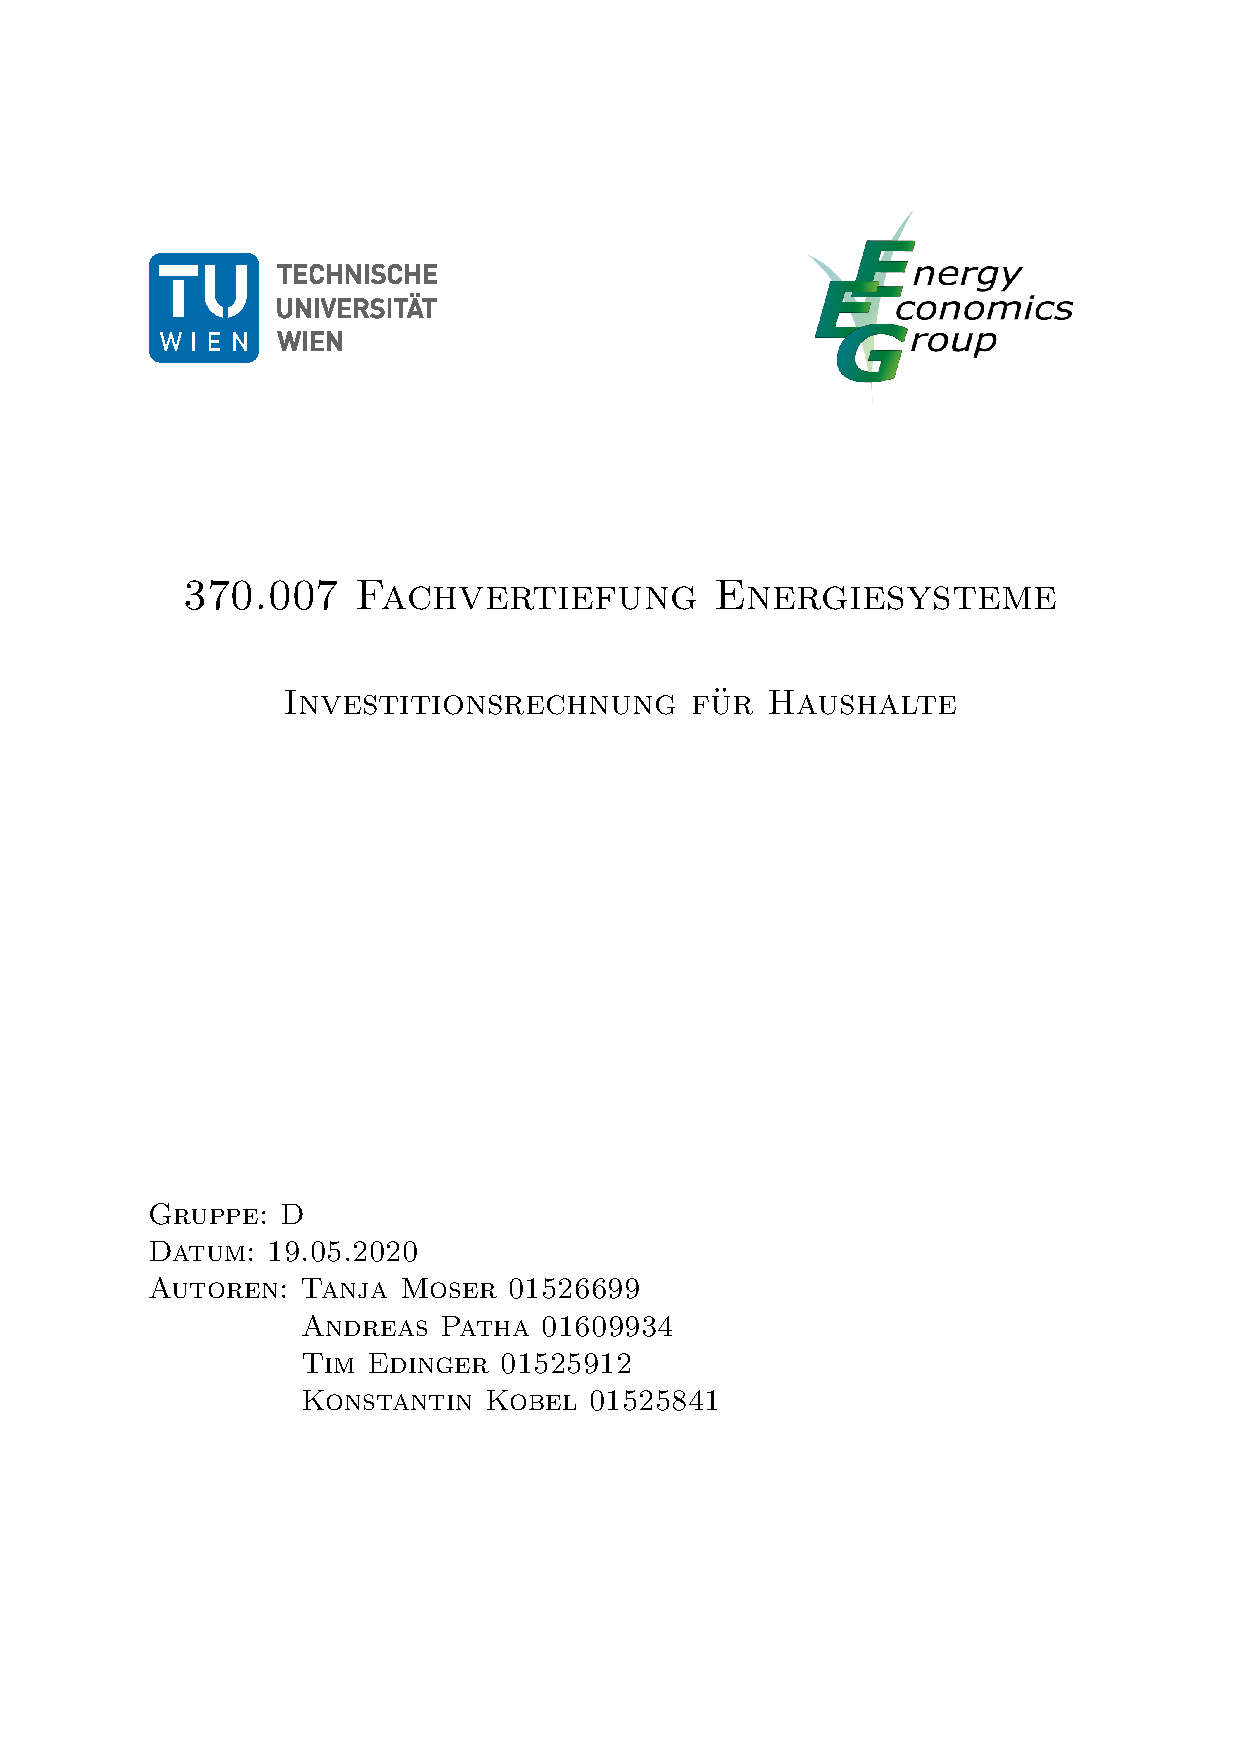
\includepdf{Protokoll_titlepage.pdf}

	\newpage
	\tableofcontents

	\newpage
	\section{Aufgabenstellung}
	Das Ziel der dritten Übung ist es, die Wirtschaftlichkeit einer PV-Anlage, für einen Haushalt, zu errechnen.\newline
	Die einzelnen Aspekte werden in drei Aufgaben behandelt.
	\subsection{Aufgabe 3.1}
	Aufgabe 3.1 befasst sich mit dem Barwert (= dem Kapitalwert) einer $10kWp$ PV-Anlage.\newline
	In dieser ersten Aufgabe wird davon ausgegangen, dass die gesamte Produktion verkauft wird.\\ \par
	\noindent Zur Berechnung werden folgende \textbf{Parameter} definiert:
	\begin{itemize}
		\item Der Zinssatz beträgt $4\%$.
		\item Die Systemkosten betragen $1200\mbox{\euro}/kWp$.
		\item Die Betriebskosten/die Versicherung belaufen sich auf $4\mbox{\euro}/(kWp\,a)$.
		\item Die Lebensdauer der PV-Anlage kann mit $25$ Jahren angenommen werden.
		\item Der $Einspeisetarif_{OeMAG}$ beträgt $8.24\,Cent/kWh$.
		\item Die $F\ddot{o}rderdauer_{OeMAG}$ beträgt $13$ Jahre.
		\item Die relevanten Spotpreise werden in der Datei $Spotpreise.mat$ zur Verfügung gestellt.
		\item Informationen zu Förderungen können folgendem Link entnommen werden:\newline
		\url{http://www.oem-ag.at/de/foerderung/photovoltaik/}
	\end{itemize}
	Es werden folgende \textbf{Annahmen} getroffen:
	\begin{itemize}
		\item Das Jahr 2016 steht exemplarisch für jedes kommende Jahr.
		\item Auch nach dem Vertragsende wird der Strom, bis zum Ende der Lebensdauer, am Spotmarkt verkauft. Die Preise entsprechen dabei den Preisen aus dem Jahr 2016.
	\end{itemize}
	Die \textbf{Aufgaben} lauten:
	\begin{itemize}
		\item[a)] Berechnen Sie den Barwert (= Kapitalwert) einer 10 kWp PV-Anlage unter der Annahme, dass die gesamte Produktion am Spotmarkt verkauft wird.
		\begin{itemize}
			\item Wie hoch dürfen die Investitionskosten maximal sein, damit die Wirtschaftlichkeit der Investition positiv bewertet wird (Barwert > 0)?
			\item Stellen Sie die Entwicklung des Kapitalwerts (=Barwert) der Investition über die Lebensdauer in einem Diagramm dar.
		\end{itemize}
		\item[b)] Führen Sie die Berechnung noch einmal unter der Annahme durch, dass Sie den aktuellen OeMAG Einspeisetarif für 13 Jahre erhalten.\newline Vergleich Sie diesen Fall mit dem nicht geförderten Fall.
	\end{itemize}
	\subsection{Aufgabe 3.2}
	In Aufgabe 3.2 wird der Eigenverbrauch der Haushalte berücksichtigt und nur noch der Überschuss der Produktion verkauft.\\ \par
	\noindent Folgende \textbf{Parameter} sind gegeben:
	\begin{itemize}
		\item Es handelt sich um eine $5kWp$ PV-Anlage.
		\item Das Einspeiseprofil der PV-Anlage wird in der Datei $PV_Einspeiseprofil.mat$ zur Verfügung gestellt.
		\item Der Standort der PV-Anlage ist Wien.
		\item Die Ausrichtung der PV-Anlage ist mit einem Azimut von $180^{\circ}$ und einem Neigungswinkel von $30^{\circ}$ gegeben.
		\item Die benötigte Leistung der Haushalte ist in der Datei $LeistungHaushalte.mat$ definiert.
	\end{itemize}
	Die \textbf{Aufgaben} lauten:
	\begin{itemize}
		\item[a)] Berechnen Sie den Eigenverbrauch und die Überschusseinspeisung einer $5kWp$-Anlage für 5 der gegebenen 30 Haushalte.
		\item[b)] Stellen Sie die Entwicklung des Eigenverbrauchsanteils und der Deckungsgrade der Haushalte für eine Anlagengröße von $0kWp$ bis $20kWp$ für die 5 Haushalte dar.
		\item[c)] Erstellen Sie eine Grafik, in der die Erzeugung, die Last und der Eigenverbrauch für die Woche 3 und 25 für Haushalt 1 dargestellt wird. Verwenden Sie für die Darstellung des Eigenverbrauchs die Plot-Funktion $area$.
	\end{itemize}
	\subsection{Aufgabe 3.3}
	In Aufgabe 3.3 sollen die Berechnungen von Aufgabe 3.2 erweitert werden.\\ \par
	\noindent Dazu werden folgende \textbf{Annahmen} getroffen:
	\begin{itemize}
		\item Für den Eigenverbrauch kann eine Ersparnis in Höhe des Haushaltsstrompreises angesetzt werden. Diese beträgt $15\,Cent/kWh$.
		\item Für die Überschusseinspeisung kann ein Einspeisetarif von $5\,Cent/kWh$ angenommen werden.
	\end{itemize}
	Die \textbf{Aufgaben} lauten:
	\begin{itemize}
		\item[a)] Erstellen Sie eine Investitionsrechnung (Barwert) für die 5 gegebenen Haushalte und einer Anlagengröße von $5kWp$. Vergleichen Sie dazu den Fall mit PV-Anlage mit dem Fall ohne PV-Erzeugung.
		\item[b)] Wie hoch dürfen die spezifischen Investitionskosten (EUR/kW) je Haushalt maximal sein, damit die Investition als wirtschaftlich gewertet wird?
	\end{itemize}
	\subsection{Aufgabe 3.4}
	In Aufgabe 3.4 soll eine Beurteilung von PV-Anlagen in Österreich, auf Basis der in den vorigen Aufgaben durchgeführten Berechnungen, getroffen werden.\\ \par
	\noindent Die \textbf{Fragen} lauten:
	\begin{itemize}
		\item[a)] Erstellen Sie eine Investitionsrechnung (Barwert) für die 5 gegebenen Haushalte und einer Anlagengröße von $5kWp$. Vergleichen Sie dazu den Fall mit PV-Anlage mit dem Fall ohne PV-Erzeugung.
		\item[b)] Wie hoch dürfen die spezifischen Investitionskosten (EUR/kW) je Haushalt maximal sein, damit die Investition als wirtschaftlich gewertet wird?
	\end{itemize}
	\newpage
	\section{Berechnungen}
	\subsection{Temperaturabhängigkeit einer PV-Anlage}

	\section{Ergebnisse}

	\newpage
	\section{Literatur}
	\begin{itemize}
		\item Literatur 1
	\end{itemize}
	\listoffigures
\end{document}